%!TEX root = ../Thesis.tex
\section{Prototypisches Beispiel in Angular}\label{sec:PrototypischesBeispiel}

In diesem Kapitel wird ein prototypisches Beispiel beschrieben, auf welches sich die im nachfolgenden \cref{sec:Evaluierung} stattfindende Evaluierung beziehen wird. Das Ergebnis der Evaluierung wird im darauffolgenden \cref{sec:Implementierung} angewendet, um die Ergebnisse zu verifizieren.

Zum Verständnis des Prototypen wird in den nachfolgenden Abschnitten zunächst die Architektur in einer Schichtenansicht präsentiert und anschließend detaillierter auf die Portalshell sowie die eingebundenen Microfrontends eingegangen. Zuletzt werden in \cref{sec:PrototypAnforderungen} die Anforderungen der Microfrontends für die Einbindung in die Portalshell konkret benannt, damit diese in der Evaluierung im darauffolgendem Kapitel berücksichtigt werden können.

\textbf{Szenario des Beispieles}\\
Bei der nachfolgend beschriebenen Beispielapplikation handelt es sich um eine Portalshell, welche im \gls{B2B}-Kontext verwendet wird. Firmenkunden wird Zugang zu der Portalshell gewährt und diese können über die Softwarelösung ihre Backoffice Tätigkeiten erledigen. Die Portalshell ist mandantenfähig, denn jeder \gls{B2B} Kunde soll individuell konfigurierte Microfrontends nutzen können. 

Damit die Portalshell nicht bei jedem hinzugefügten Microfrontend jedes Mandanten neu veröffentlicht werden muss, ist das Anzeigen der Microfrontends dynamisch gelöst. Es werden von den Usern die individuellen Konfigurationen und Anordnungen der Microfrontends zur Laufzeit geladen. Als Beispiel möchte Kunde A auf der Startseite ein Microfrontend zum Ticketmanagement angezeigt bekommen. Kunde B hingegen benötigt auf der Startseite zwei konfigurierte \gls{KPI}s sowie ein Microfrontend zur Suche auf dem eigenen Fileshare.

Die Portalshell bietet den Microfrontends, welche auch teilweise vom \gls{B2B} Kunden selber entwickelt werden, die Möglichkeit auf Querschnittsaspekte des Portals zuzugreifen. Darunter fallen beispielsweise Logging, Lokalisierung, Benutzer- und Mandanteninformationen, Autorisierung und das Laden von Konfigurationswerten. Die Portalshell wird von mandantenunabhängigen Administratoren übergreifend verwaltet. Sie können neue Microfrontends registrieren, User anlegen und diese zu Mandanten zuweisen sowie einen First-Level-Support stellen. Die Administratoren sind ebenfalls für den Betrieb der Portalshell zuständig und Hosten diese in Azure.

In den nachfolgenden Abschnitten wird die Architektur sowie Details zu drei prototypischen Microfrontends für einen Mandanten im Detail präsentiert.

\subsection{Architekturübersicht}\label{sec:PrototypArchitekturdiagramm}

In der nachfolgenden Abbildung \cref{fig:ArchitekturBsp} ist die beispielhafte Microfrontendarchitektur dargestellt und in die Schichten Frontend, Backend und Datenbank getrennt. 

\begin{figure}[hbt!]
	\centering
	\begin{minipage}[t]{0.8\textwidth}	
		\caption{Beispielapplikation Microfrontend-Architektur}
		\frame{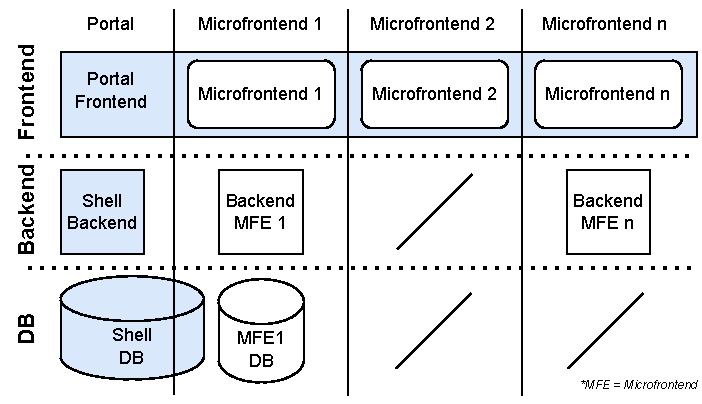
\includegraphics[width=1\textwidth, page=1]{img/Beispielapplikation_Diagramm}}\\ % Pfad
		\source{Eigene Darstellung} % Quelle
		\label{fig:ArchitekturBsp}
	\end{minipage}
\end{figure}

Die Applikation besteht aus einer Portalshell, zu welcher ein Frontend, ein Backend sowie eine Datenbank gehört. In das Frontend der Portalshell sind mehrere Microfrontends eingebunden, welche entweder aus einem Frontend mit einem eigenen Backend sowie einer eigenen Datenbank bestehen (siehe \gls{MFE1}), nur aus einem Frontend bestehen (siehe \gls{MFE2}) oder aus einem Frontend und einem Backend bestehen (siehe Microfrontend n).

Das Backend der Portalshell sowie das Backend des \gls{MFE1} greifen jeweils auf die Datenbank der Portalshell zu (siehe nachfolgende \cref{fig:SolutionarchitekturBsp}). Die Portalshell verwaltet die Nutzer und deren Berechtigungen. Sie stellt Schnittstellen bereit, damit Microfrontends die Nutzerinformationen bei Bedarf konsumieren können.

\newpage
\begin{figure}[hbt]
	\centering
	\begin{minipage}[t]{0.6\textwidth}	
		\caption{Beispielapplikation Solutionarchitektur}
		\frame{\includegraphics[width=1\textwidth,page=2]{img/Beispielapplikation_Diagramm}}\\ % Pfad
		\source{Eigene Darstellung} % Quelle
		\label{fig:SolutionarchitekturBsp}
	\end{minipage}
\end{figure}

Die Portalapplikation verfügt über ein Rollenkonzept. Die Rollen werden für jeden User pro Microfrontend vergeben. Das Microfrontend 1 fragt die \gls{DB} der Portalshell nach der Rolle des aktuellen Users ab, weil es diese Information zum Anzeigen der Inhalte benötigt. Bei Microfrontend n und \gls{MFE2} haben alle Benutzer die gleichen Rechte, weswegen Abfragen der Rollen nicht nötig sind. Das \gls{MFE2} fragt in regelmäßigen Abständen eine öffentliche \gls{API} an und zeigt die Ergebnisse der Anfrage aufbereitet im Frontend an.

\subsection{Portalapplikation}\label{sec:PrototypPortalapplikation}

Die Portalapplikation basiert auf dem Angular Framework und bietet, wie in \cref{sec:Portalapplikationen} beschrieben, einige Querschnittsaspekte.

So ist Authentifizierung sowie die generelle Benutzerverwaltung über das Portal abgedeckt. Für Benutzer muss, bevor sie sich im Portal anmelden können, ein Account zum Einloggen sowie eine dazugehörige Rollenzuweisung angelegt werden. Es sind zwei Rollen verfügbar, welche in der \cref{tab:RollenPortalapplikation} in Anhang \ref{app:Tabellen} mit ihrer jeweiligen Funktion dargestellt sind.

Eine Rollenzuweisung stellt die Verbindung zwischen einem Benutzer und einem Mandanten her. Ein Benutzer kann in mehreren Mandanten jeweils eine Rolle zugewiesen bekommen. Eine Übersicht der zusammenhängenden Elemente in der Portalapplikation ist in der nachfolgenden \cref{fig:NutzerMandantenDashboard} zu sehen.

\begin{figure}[hbt!]
	\begin{minipage}[t]{1\textwidth}	
		\caption{Übersicht der Elemente der Portalshell}
		\frame{\includegraphics[width=1\textwidth, page=4]{img/Beispielapplikation_Diagramm}}\\ % Pfad
		\source{Eigene Darstellung} % Quelle
		\label{fig:NutzerMandantenDashboard}
	\end{minipage}
\end{figure}

In dem Portal können Microfrontends dynamisch eingebunden werden. Es gibt eine Oberfläche, auf der Administratoren des Portals neue Microfrontends konfigurieren können. Zu jedem Microfrontend wird ebenfalls die Konfiguration der Parameter des Microfrontends gespeichert. Microfrontends können anschließend instanziiert werden, indem sie einem Mandanten zugewiesen und die Parameter-Konfigurationen auf die Werte des Mandanten gesetzt werden. So können die Microfrontends dynamisch für verschiedene Mandanten gleichzeitig genutzt werden. Eine Übersicht der Elemente mit beispielhaften Ausprägungen ist zur besseren Verständlichkeit in Anhang \ref{app:Bilder} in \cref{fig:PortalapplikationElementeKonkret} dargestellt.

Ein Dashboard bezeichnet eine für einen Mandanten individuell konfigurierte Anordnung von Microfrontendinstanzen, auf die Benutzer eines Mandanten zugreifen können. Die einzelnen Microfrontendinstanzen können für den eingebunden Mandanten individuell konfiguriert sein. Liegt keine Konfiguration vor, wird entweder auf einen Standardwert des Microfrontend-Templates zurückgegriffen oder ganz auf Konfiguration verzichtet.

Die Nutzer eines Mandanten können sich die eingebundenen Microfrontendinstanzen individuell auf dem Dashboard konfigurieren, wie es zum Beispiel auch bei Azure Dashboards der Fall ist.\footnote{\cite[vgl.][]{Microsoft2021a}} Die Portalshell stellt Dialoge zum Registrieren und Verwalten von Dashboards für einen Mandanten zur Verfügung.

Damit die Portalapplikation sowie die eingebundenen Microfrontends integriert werden können und dem gleichen Design folgen, wird ein \gls{SDK} zur Verfügung gestellt. Dieses beinhaltet Formularelemente, wie beispielsweise Buttons, interaktive Textboxen oder Dropdownlisten. Diese Formularelemente sind einheitlich gestylt und können miteinander interagieren, um clientseitige Validierung zu ermöglichen.

Ebenfalls sorgt die Portalshell für Fehlerbehandlung, sollte ein Microfrontend in einem Dashboard nicht geladen werden können. In diesem Fall wird ein Platzhalter mit entsprechendem Text angezeigt und der Fehler protokolliert, damit das Entwicklerteam reagieren kann. Auch bietet das Portal eine Schnittstelle, damit eingebundene Microfrontends etwaige Fehler zentral protokollieren können.

\subsection{Eingebundene Microfrontends}\label{sec:PrototypMicrofrontends}

In die im vorherigen Abschnitt beschriebene Portalapplikation werden Microfrontends eingebunden. Um ein Microfrontend einbinden zu können, muss dieses vorher im Portal mit den Parametern \gls{URL}, Art der Einbindung und optionalen mandantenindividuellen Konfigurationen registriert werden. Es entsteht ein Template des Microfrontends, welches nur die Hosting-Parameter sowie die Schlüssel der Konfigurationen enthält. Die Ausprägungen der Konfigurationen werden bei der Instanziierung des Microfrontends zu einem Mandanten gesetzt. Anschließend lädt die Portalshell die Konfiguration der Microfrontendinstanz dynamisch aus der Datenbank, damit sie nicht immer bei jeder Änderung an den konfigurierten Microfrontends neu veröffentlicht werden muss.

Im Fall der in \cref{fig:ArchitekturBsp} beschriebenen Architektur handelt es sich bei \gls{MFE2} um eine Wetter-Applikation, welche regelmäßig eine Wetter-\gls{API} aufruft. Für jeden Mandanten ist der Standort als Parameter der Microfrontendinstanz konfiguriert, sodass das Wetter des Standortes angezeigt wird, an welchem der Mandant sich befindet. Exemplarisch soll für den prototypischen Mandanten das Wetter von zwei Standorten angezeigt werden, da Benutzer das Wetter an ihrem Arbeitsplatz, aber auch von ihrer Heimatstadt verfolgen können sollen. Von dem Wetter-Microfrontend werden dementsprechend zwei Instanzen mit unterschiedlichen Parametern eingebunden.

Microfrontend n ist eine Taschenrechner App, welche von allen Usern genutzt werden darf. Die Taschenrechner-App verfügt über keine Parameter und ist für alle Mandanten gleich.

Microfrontend 1 stellt eine Statistik App dar. Diese darf von allen Benutzern angezeigt werden. Normale Benutzer sehen die App mit verringertem Umfang. Nutzer mit der Administrator-Rolle sehen erweiterte Statistiken, die sonst nicht sichtbar sind. Die Statistik-App fragt die Portalapplikation an, ob der Benutzer ausreichend Rechte hat, um den Administrator-Bereich der Statistik-App einsehen zu dürfen. Dafür muss die Statistik-App Informationen über den aktuellen Benutzer kennen, wie beispielsweise seinen Namen und eine eindeutige Kennung.

Die externen Abhängigkeiten der Microfrontends sind in einer Solutionarchitektur  dargestellt, welche in Anhang \ref{app:Bilder} in \cref{fig:SolutionarchitekturBeispielapplikationKonkret} abgebildet ist.

Ein Mockup des Designs von der Portalshell mit den vier eingebundenen Microfrontendinstanzen auf einem Dashboard mit dem Namen \textit{Prototyp} ist in der nachfolgenden \cref{fig:MockupBeispiel} dargestellt. Die blauen Balken links und oben werden von der Portalshell gestellt. Links an der Seite befindet sich die Navigation, durch die zwischen Dashboards gewechselt werden kann. Oben im Header sind Informationen zum Mandanten sowie ein Icon sichtbar, auf welches der Benutzer zum Verwalten seines Profils und zum Abmelden klicken kann.

\begin{figure}[hbt!]
	\centering
	\begin{minipage}[t]{0.7\textwidth}	
		\caption{Design Mockup Dashboard \textit{Prototyp}}
		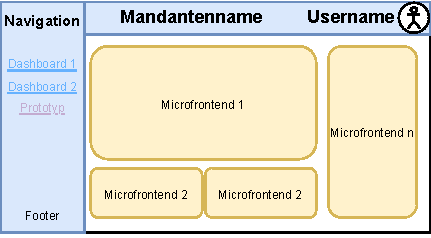
\includegraphics[width=1\textwidth]{img/MockupBeispiel}\\ % Pfad
		\source{Eigene Darstellung} % Quelle
		\label{fig:MockupBeispiel}
	\end{minipage}
\end{figure}

Der restliche in weiß dargestellte Bereich der rechteckigen Anwendung ist der Platzhalter des ausgewählten Dashboards. Die vier eingeblendeten Microfrontendinstanzen entstammen drei konfigurierten Microfrontend-Templates.

\subsection{Anforderungen an das System}\label{sec:PrototypAnforderungen}

Nach dem Definieren der Portalapplikation sowie den eingebundenen Microfrontends können konkrete Anforderungen gestellt werden, welche die Art der Einbindung erfüllen sollte.

Durch das in \cref{fig:NutzerMandantenDashboard} aufgezeigte und in \cref{sec:PrototypMicrofrontends} beschriebene Konzept der Konfigurierbarkeit der Microfrontends muss bei der Art der Einbindung eine Möglichkeit bestehen, Parameter übergeben zu können. Ansonsten wäre eine mandantenfähige Portalapplikation nicht zu realisieren.

Da die \gls{UX} das Erlebnis des Benutzers auf der Webseite beschreibt, spielt sie eine relevante Rolle. So sollten Portalapplikation und Microfrontends ein einheitliches Design haben und insgesamt über geringe Ladezeiten verfügen.

Weiterhin soll der Benutzer nach Möglichkeit im Portal bleiben und nicht zwischen verschiedenen Webseiten wechseln müssen. Es soll sich anfühlen, als wäre er durchgehend nur in der Portalapplikation unterwegs. Softes Routing sollte der Standardfall sein.\newline
In sinnvollen Ausnahmefällen, beispielsweise bei einem Klick auf \textit{Mail senden}, dürfte auch ein hartes Routing in ein anderes Programm erfolgen. Ebenfalls soll es möglich sein mehrere Microfrontends auf einer Seite einzubinden. 
Der Nutzer muss in der Lage sein, sich die Dashboards individuell anzupassen und dort unter Umständen auch viele Instanzen des gleichen Microfrontends mit unterschiedlichen Parametern nebeneinander darzustellen.

Zusammengefasst sind für die exemplarische Angular Portalapplikation und die dazugehörigen eingebundenen Microfrontends die Aspekte Parameterübergabe, einheitliches Design, eingebundene Navigation und geringe Ladezeiten wichtig.